\section{Fremderregte Schwingung}

\subsection{Definition}

Erzwungene Schwingungen sind Schwingungen, die durch eine \textbf{periodische Störung} verursacht werden.


\subsection{Übersicht über Hilfsgrössen}

\renewcommand{\arraystretch}{2.6}
\begin{ctabular}{|cc c cc|}
    \hline
    $\omega_0 = \sqrt{\dfrac{k}{m}}$     & & $\delta = \dfrac{\kappa}{2} = \dfrac{b}{2 \, m}$    & & $ D = \dfrac{\delta}{\omega_0} =  \dfrac{\kappa}{2 \, \omega_0}$            \\
    $\eta = \dfrac{\omega}{\omega_0}$    & & \multicolumn{3}{c|}{$\Omega_d = \sqrt{\omega_0^2 - \delta^2} =  \omega_0 \sqrt{1 - D^2}$}     \\
    \hline
\end{ctabular}


\renewcommand{\arraystretch}{1.5}
\begin{ctabular}{c l c}
    $\omega_0$                  & Kreisfrequenz ungedämpfte Schwingung  & $[\omega_0] = \frac{\rad}{\second}$       \\
    $\Omega_d$                  & Kreisfrequenz gedämpfte Eigenfrequenz & $[\Omega_d] = \frac{\rad}{\second}$       \\
    $\omega_r$                  & Resonanzkreisfrequenz                 & $[\omega_r] = \frac{\rad}{\second}$       \\
    $\omega$                    & Kreisfrequenz der Störung (Erreger)   & $[\omega] = \frac{\rad}{\second}$         \\
    $\delta = \frac{\kappa}{2}$ & Abklingkonstante                      & $[\kappa] = [\delta] = \frac{1}{\second}$ \\
    $D$                         & Dämpfungsgrad                         & $[D] = 1$                                 \\
    $\eta$                      & Dimensionslose Frequenz               & $[\eta] = 1$                              \\
    $k = c$                     & Federkonstante                        & $[k] = \frac{\newton}{\meter}$
\end{ctabular}
\renewcommand{\arraystretch}{1}


\subsection{Resonanz}

Die Amplitude $A$ wird maximal, wenn der Nenner von $A(\omega)$ minimal wird.

\begin{minipage}{0.48\columnwidth}
    $$ \boxed{ \omega_r = \omega_0 \sqrt{1 - 2 \, D^2} } $$
\end{minipage}
\hfill
\begin{minipage}{0.48\columnwidth}
    $$ \boxed{ A_r = \frac{u_0}{2 \, D \sqrt{1 - D^2}} }$$
\end{minipage}


\subsection{Fremderregte Schwingung -- Krafterregung}

\begin{center}
    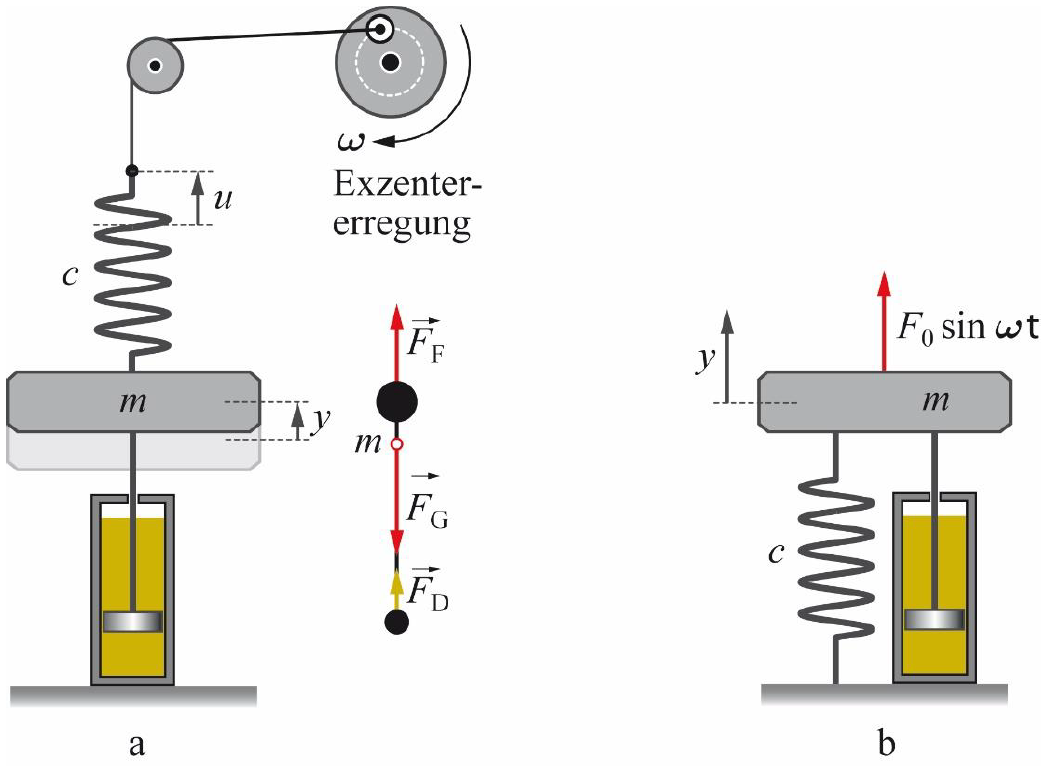
\includegraphics[width=0.75\columnwidth]{images/krafterregung.png}
\end{center}

\vspace{-0.3cm}

$$ \boxed{ \text{DGL:} \quad m \, \ddot{y} + b \, \dot{y} + c \, y = F_0 \, \sin(\omega \, t) } $$  

$$ y(t) = \underbrace{ A(\omega) \, \sin(\omega \, t - \varphi) }_{\substack{y_p(t)}} + \underbrace{ B \, e^{- \delta t} \sin(\Omega_d \, t + \varphi_0)}_{\substack{y_h(t)}} $$


\begin{minipage}[c]{0.3\columnwidth}
    $$ \boxed{ \varphi = \arctan \left( \frac{2 \, D \, \omega_0 \, \omega}{\omega_0^2 - \omega^2} \right) } $$
\end{minipage}
\hfill
\begin{minipage}[c]{0.68\columnwidth}
    $$ \boxed{ A(\omega) = \frac{F_0}{m \sqrt{(\omega_0^2 - \omega^2)^2 + (2 \, D \, \omega_0 \, \omega)^2 } } } $$
\end{minipage}


\subsubsection{Vergrösserungsfunktion / Phasenverschiebung}
\label{Vergrösserungsfunktion / Phasenverschiebung}

\vspace{-0.2cm}

\[
    \boxed{ V = \frac{1}{\sqrt{(1- \eta^2)^2 + (2 \, D \, \eta)^2} } }
    \qquad \qquad
    \boxed{ \varphi = \arctan \left( \frac{2 \, D \, \eta}{1 - \eta^2}  \right) }
\]
$$ \boxed{ V_r = \frac{1}{\sqrt{ 1 - \eta_r^4} } \qquad \text{mit } \eta_r = \sqrt{1 - 2 \, D^2} } $$


\begin{ctabular}{c l c}
    $\varphi$   & Phasenverschiebung                    & $[ \varphi] = \rad$                   \\
    $V$         & Vergrösserungsfunktion                & $[V] = 1$                             \\
    $V_r$       & Vergrösserungsfunktion                & $[V_r] = 1$                           \\
    $\eta$      & Dimensionslose Frequenz               & $[\eta] = 1$                          \\
    $D$         & Dämpfungsgrad                         & $[D] = 1$                             \\
    $A(\omega)$ & Amplitudenverlauf                     & $[A(\omega)] = \meter$                \\
    $\varphi$   & Phasenverschiebung                    & $[\varphi] = \rad$                    \\
    $\omega_0$  & Kreisfrequenz ungedämpfte Schwingung  & $[\omega_0] = \frac{\rad}{\second}$   \\
    $\omega$    & Kreisfrequenz der Störung (Erreger)   & $[\omega] = \frac{\rad}{\second}$     \\
\end{ctabular}


\subsection{Fremderregte Schwingungen -- Dämpfererregung}

\begin{minipage}[t]{0.21\columnwidth}
    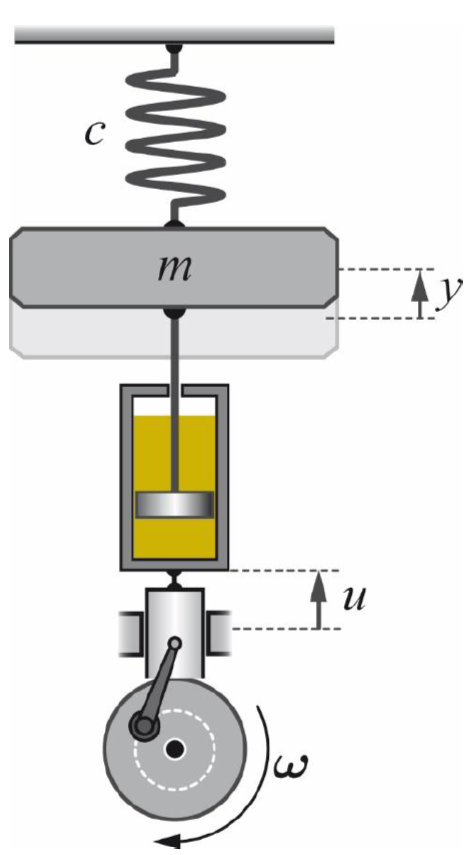
\includegraphics[width=\columnwidth, align=t]{images/daempfererregung.png}
\end{minipage}
\hfill
\begin{minipage}[t]{0.71\columnwidth}
    $$ \boxed{ \text{DGL:} \quad m \, \ddot{y} + b \, \dot{y} + c \, y = b \, \omega  \, u_0 \, \cos(\omega \, t) } $$ 
    $$ A(\omega) =  \frac{b \, \omega \, u_0}{ m \sqrt{(\omega_0^2 -\omega^2)^2 + (2D \omega_0 \omega)^2}} $$ 

    \[
        \boxed{ V = \frac{2 \, D \, \eta}{\sqrt{(1- \eta^2)^2 + (2 \, D \, \eta)^2} } }
        \qquad 
        \boxed{ \varphi = \arctan \left( \frac{2 \, D \, \eta}{1 - \eta^2} \right) - \frac{\pi}{2} }
    \]

    \textrightarrow\ Legende siehe Abschnitt \ref{Vergrösserungsfunktion / Phasenverschiebung}
\end{minipage}


\subsection{Fremderregte Schwingungen -- Stützenerregung}

\begin{minipage}[t]{0.22\columnwidth}
    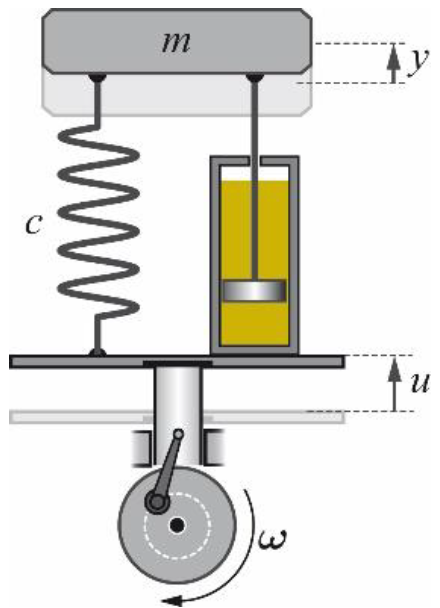
\includegraphics[width=\columnwidth, align=t]{images/stuetzenerregung.png}
\end{minipage}
\hfill
\begin{minipage}[t]{0.7\columnwidth}
    $$ \boxed{ \text{DGL:} \quad m \, \ddot{q} + b \, \dot{q} + c \, q = -m \, \omega^2 \, u_0 \, \sin(\omega \, t)  \quad \text{mit } q = y - u } $$
    $$ A(\omega) = \frac{\omega^2 u_0}{\sqrt{(\omega_0^2 -\omega^2)^2 + (2 \, D \, \omega_0 \, \omega)^2}} $$ 

    \[
        \boxed{ V = \frac{\eta^2}{\sqrt{(1- \eta^2)^2 + (2 \, D \, \eta)^2} } }
        \qquad 
        \boxed{ \varphi = \arctan \left( \frac{2 \, D \, \eta}{1 - \eta^2} \right) - \pi }
    \]

    \textrightarrow\ Legende siehe Abschnitt \ref{Vergrösserungsfunktion / Phasenverschiebung}
\end{minipage}



\subsection{Fremderregte Schwingung -- Unwuchterregung}
\textbf{Unwucht:} Schwerpunkt $S$ des Rotors der Masse $m_R$ bewegt sich auf einem Kreis mit\\
Radius $e$

\begin{minipage}[t]{0.52\columnwidth}
    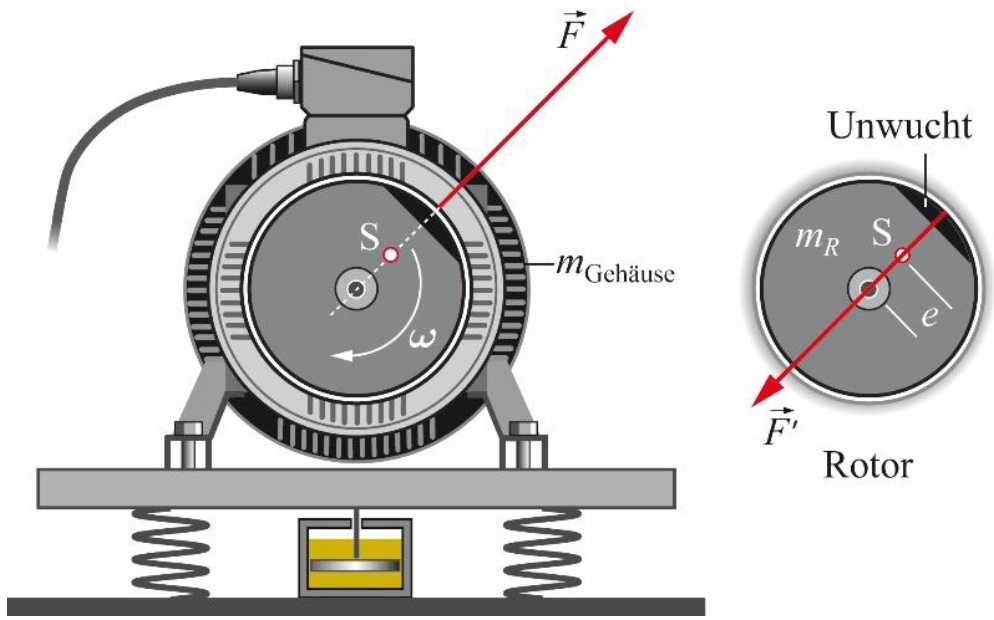
\includegraphics[height=3cm, align=t]{images/unwucht.png}
\end{minipage}
\hfill
\begin{minipage}[t]{0.44\columnwidth}
    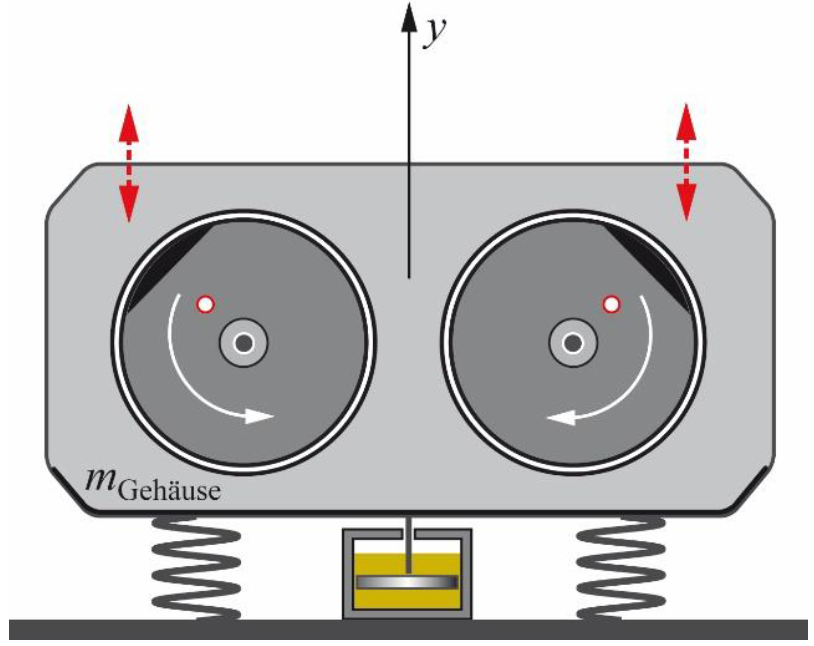
\includegraphics[height=3cm, align=t]{images/unwucht_gehause.png}
\end{minipage}

\smallskip

$$ \boxed{ \text{DGL in y-Richtung:} \quad m \ddot{y} + b \dot{y} + c \, y = -m_R \, \omega^2 \, e \, \sin(\omega \, t) }  $$

\renewcommand{\arraystretch}{1,7}
\begin{tabular}{ll}
    Radiale Beschleunigung des Schwerpunkts des Rotors: & $a_R = \omega^2 e$                                    \\
    Kraft des Rotors auf die Maschine:                  & $\boxed{ F_U = m_R \cdot a_R = m_R \cdot \omega^2 e }$ 
\end{tabular}
\renewcommand{\arraystretch}{1}

\medskip

\[
    A(\omega) = \frac{m_R}{m} \frac{e \, \omega^2}{\sqrt{(\omega_0^2 -\omega^2)^2 + (2 \, D \, \omega_0 \, \omega)^2}} 
    \qquad \qquad
    A_R = \frac{m_R}{m} \frac{e}{2 \, D \sqrt{1 - D^2}}
\]


\subsubsection{Kraft auf die Basis des Gehäuses} 

\vspace{-0.5cm}

\[
    F_B = c y + b \dot{y} = F_{B0} \sin(\omega t - \varphi + \psi)
    \qquad 
    \varphi = \psi - \pi
    \qquad 
    \boxed{ F_{B0} = \frac{m_R \, e \, \omega^2 \sqrt{1+ (2D \eta)^2}}{\sqrt{(1 - \eta^2)^2 + (2 D \eta)^2}} }
\]


\begin{ctabular}{c l c}
    $F_{B0}$    & Kraft auf Basis des Gehäuses          & $[F_{B0}] = \newton$              \\
    $m_R$       & Masse des Rotors                      & $[m_R] = \kilogram$               \\
    $a_R$       & Radiale Beschleinigung Schwerpunkt    & $[a_R] = \frac{\meter}{\second}$  \\
    $e$         & Abstand Mittelpunkt - Schwerpunkt     & $[e] = \meter$                    \\
    $\varphi$   & Phasenverschiebung                    & $[ \varphi] = \rad$               \\
    $V$         & Vergrösserungsfunktion                & $[V] = 1$                         \\
    $\eta$      & Dimensionslose Frequenz               & $[\eta] = 1$                      \\
    $D$         & Dämpfungsgrad                         & $[D] = 1$                         \\
    $A(\omega)$ & Amplitude                             & $[A(\omega)] = \meter$            \\
    $A_R$       & Resonanzamplitude                     & $[A_R] = \meter$
\end{ctabular}


\subsection{Fremderregte Schwingung -- Schwingkreis}

\begin{minipage}[t]{0.4\columnwidth}
    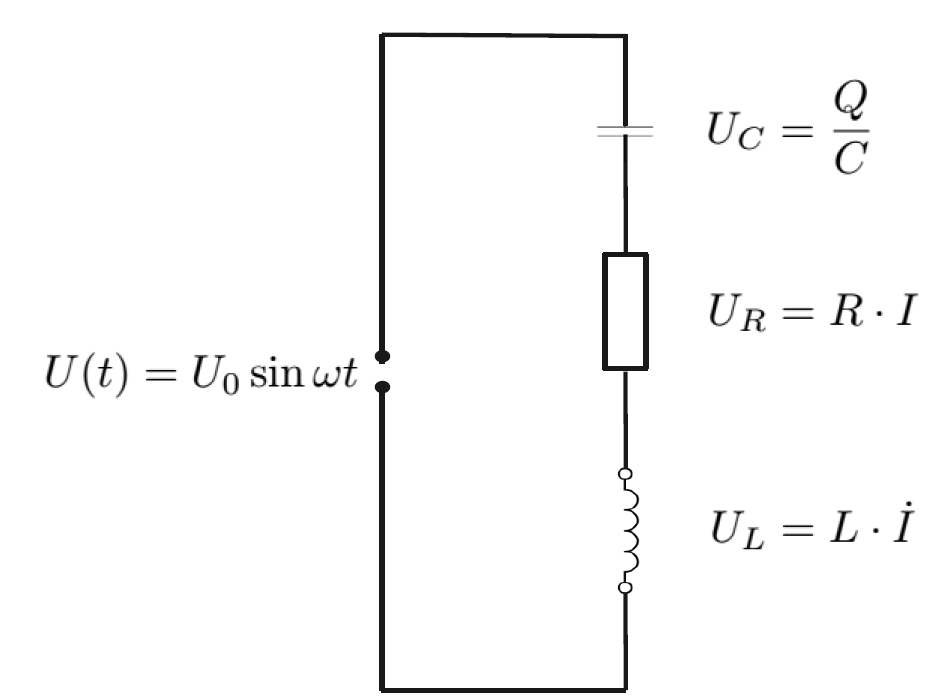
\includegraphics[width=\columnwidth, align=t]{images/schwingkreis.png}
\end{minipage}
\hfill
\begin{minipage}[t]{0.58\columnwidth}
    $$ \boxed{ \text{DGL:} \quad L \ddot{I} + R \dot{I} + \frac{1}{C} \, I = \omega \, U_0 \,\sin \left( \omega \, t + \frac{\pi}{2} \right) } $$
    \textrightarrow\  Gleiche DGL wie bei \cbl{Dämpfererregung}

    $$ \cbl{\text{DGL:} \quad m \ddot{y} + b \dot{y} + c \, y = b \, \omega \, u_0 \, \cos(\omega \, t) } $$
    $$ \cbl{A(\omega) =  \frac{b \, \omega \, u_0}{m \sqrt{(\omega_0^2 -\omega^2)^2 + (2 \, D \, \omega_0 \, \omega)^2}} } $$
\end{minipage}

\medskip

$$ \boxed{ I(\omega) =  \frac{\omega}{\sqrt{(\omega_0^2 -\omega^2)^2 + (2 \, D \, \omega_0 \, \omega)^2}} U_0 \qquad \text{mit} \quad \omega_0 = \frac{1}{\sqrt{LC}} , \quad D = \frac{R}{2}\sqrt{\frac{C}{L}}} $$ 
\[
    \boxed{ V = \frac{U_{L0}}{U_0} = \frac{\eta^2}{\sqrt{(1 - \eta^2)^2 + (2 \, D \, \eta)^2}} }
    \qquad 
    \boxed{ \varphi = \arctan \left( \frac{2 \, D \, \eta}{1 - \eta^2} \right) - \pi }
\]


\subsubsection{Resonanz}

\begin{minipage}{0.48\columnwidth}
    \paragraph{Resonanzfrequenz}
    $$ \boxed{ \omega_r = \omega_0 = \frac{1}{\sqrt{LC}} } $$ 
\end{minipage}
\hfill
\begin{minipage}{0.48\columnwidth}
    \paragraph{Amplitude @ Resonanz}
    $$ \boxed{ I_{0r} = \frac{U_0}{R} } $$ 
\end{minipage}

\renewcommand{\arraystretch}{1.3}
\begin{ctabular}{c l c}
    $\omega_0$  & Kreisfrequenz ungedämpfte Schwingung  & $[\omega_0] = \frac{\rad}{\second}$   \\
    $\omega$    & Kreisfrequenz der Störung (Erreger)   & $[\omega] = \frac{\rad}{\second}$     \\
    $\omega_r$  & Resonanzfrequenz                      & $[\omega_r] = \frac{\rad}{\second}$   \\
    $I_{0r}$    & Strom-Amplitude @ Resonanz            & $[I_{0r}] = \ampere$                  \\
    $U_0$       & Amplitude der Erregerspannung         & $[U_0] = \volt$                       \\
    $U_{L0}$    & Amplitude Spulenspannung              & $[U_{L0}] = \volt$                    \\
    $A(\omega)$ & Amplitude der Schwingung              & $[A(\omega)] = \meter$                \\
    $V$         & Vergrösserungsfunktion                & $[V] = 1$                             \\
    $\eta$      & Dimensionslose Frequenz               & $[\eta] = 1$                          \\
    $D$         & Dämpfungsgrad                         & $[D] = 1$ 
\end{ctabular}
\renewcommand{\arraystretch}{1}


\subsection[Fremderregte Schwingung -- Güte]{Fremderregte Schwingung -- Güte $Q$}

\subsubsection{Definition}

\begin{minipage}[c]{0.48\columnwidth}
    Die relative Abnahme der Schwingungsenergie $E(t)$ pro Schwingdauer wird als \textbf{Güte} oder \textbf{Gütefaktor} bezeichnet.
\end{minipage}
\hfill
\begin{minipage}[c]{0.48\columnwidth}
    $$ \boxed{ Q = 2 \pi \frac{E(t)}{E(t) - E(t + T)} } $$ 
\end{minipage}


\subsubsection{Beziehungen}

\begin{minipage}[t]{0.36\columnwidth}
    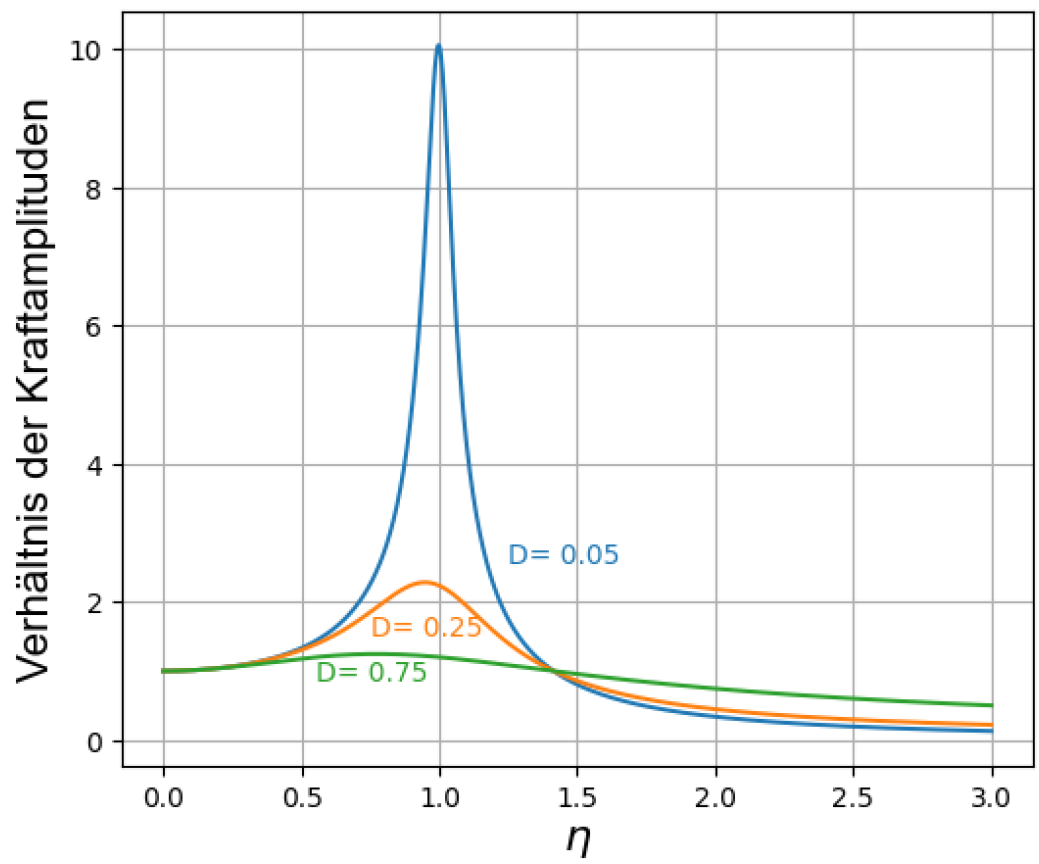
\includegraphics[width=\columnwidth, align=t]{images/guete_resonanz.png}
\end{minipage}
\hfill
\begin{minipage}[t]{0.58\columnwidth}
    \[
        \boxed{Q = \frac{1}{2 \, D} } 
        \qquad \qquad 
        \boxed{ Q = \frac{\omega_0}{\Delta \omega} }
    \]


    \medskip
    Breite der Resonanzkurve bei $U_0 = \frac{U_{0r}}{\sqrt{2}}$ \\
    \textbf{Breite Kurve \textrightarrow\  tiefe Güte}
\end{minipage}


\subsection{Gekoppelte Pendel}
Zwei Pendel sind durch eine Feder miteinander verbunden.

\textbf{Die Bewegung eines Pendels hat Auswirkungen auf die Bewegung des anderen Pendles.}
Gesucht ist eine Berschreibung der Bewegung des Pendels.

\medskip

\begin{minipage}[t]{0.28\columnwidth}
    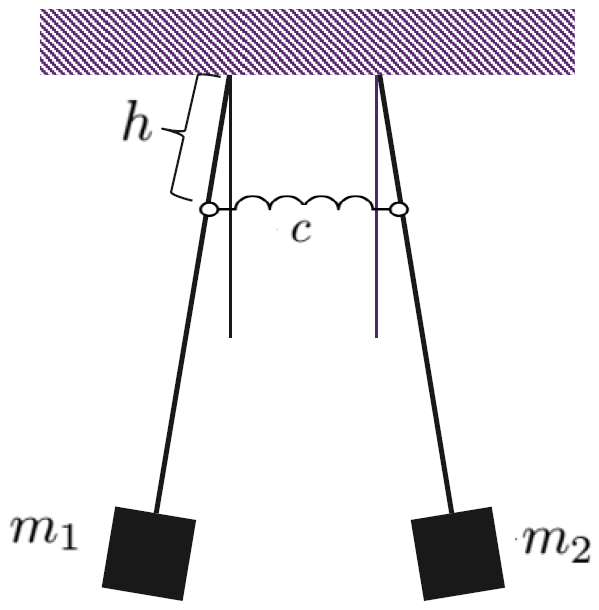
\includegraphics[width=\columnwidth, align=t]{images/gekoppelte_pendel.png}
\end{minipage}
\hfill
\begin{minipage}[t]{0.7\columnwidth}
    \paragraph{Allgemein}

    \vspace{-0.2cm}
    $$ J_1 \ddot{\varphi_1} = -m_1 \, g \, a_1 \, \varphi_1 + c \cdot h^2 \, (\varphi_2 - \varphi_1) $$
    $$ J_2 \ddot{\varphi_2} = -m_2 \, g \,  a_2 \, \varphi_2 - c \cdot h^2 \, (\varphi_2 - \varphi_1) $$

    \medskip

    \paragraph{Spezialfall}

    \begin{tabular}{lll}
        \tabitem $J_1 = J_2 = J$    & \tabitem $m_1 = m_2 = m$  & \tabitem $a_1 = a_2 = a$  \\
    \end{tabular}

    $$ \ddot{\varphi_1} = - \omega^2 \varphi_1 + k \, (\varphi_2 - \varphi_1) $$
    $$ \ddot{\varphi_2} = - \omega^2 \varphi_2 - k \, (\varphi_2 - \varphi_1) $$ 
\end{minipage}

Im Spezialfall gilt:

\vspace{-0.2cm}

\renewcommand{\arraystretch}{2}
\begin{ctabular}{lll}
    $\Phi_+ = \varphi_1 + \varphi_2$    & $\Phi_- = \varphi_2 - \varphi_1$  &                                       \\
    $\omega^2 = \dfrac{m \, g \, a}{J}$ & $k = \dfrac{c \cdot h^2}{J}$      & $\omega_k = \sqrt{\omega^2 + 2 \, k}$ \\
\end{ctabular}


\begin{ctabular}{l ll l}
    Symm:       & $\ddot{\Phi_+} = - \omega^2 \Phi_+$           & & $\varphi_1(t) = \varphi_2(t) = \dfrac{\Phi_0}{2} \cos \left( \omega t \right)$      \\
    Antisymm:   & $\ddot{\Phi_-} = - (\omega^2 + 2k) \Phi_-$    & & $\varphi_1(t) = -\varphi_2(t) = \dfrac{\Phi_0}{2} \cos \left( \omega_k t \right)$
\end{ctabular}


\subsubsection{Allgemeine Lösung des gekoppelten Systems}

\textrightarrow\ Linearkombination der symmetrischen und asymmetrischen Lösung

\vspace{-0.2cm}

\renewcommand{\arraystretch}{1.8}
\begin{ctabular}{lll}
    $\varphi_1(t) = \Phi \, \sin \left( \Omega\, t \right) \cdot \cos \left( \overline{\omega} \, t \right)$    & & $\Omega = \dfrac{\omega_k - \omega}{2}$             \\
    $\varphi_2(t) = \Phi \, \cos \left( \Omega\, t \right) \cdot \sin \left( \overline{\omega} \, t \right)$    & & $\overline{\omega} = \dfrac{\omega + \omega_k}{2}$
\end{ctabular}
\renewcommand{\arraystretch}{1}


\begin{ctabular}{c l c}
    $k$ & Kopplungsfaktor           & $[k] = 1$                                 \\
    $h$ & Abstand zur Aufhängung    & $[h] = \meter$                            \\
    $J$ & Massenträgheitsmoment     & $[J] = \kilogram \cdot \meter\squared $   \\
    $c$ & Federkonstante            & $[c] = \frac{\newton}{\meter}$
\end{ctabular}

